\documentclass[journal]{IEEEtran}

% ===== パッケージ =====
\usepackage{amsmath,amssymb}
\usepackage{graphicx}
\usepackage{booktabs}
\usepackage{cite}
\usepackage{siunitx}
\usepackage{tikz}
\usepackage{xcolor}
\usepackage{stfloats} % figure* をページ下にも置けるように

\graphicspath{{fig/}}
\DeclareGraphicsExtensions{.png,.pdf,.jpg}

% ===== 論文開始 =====
\begin{document}

\title{On-Chip Magnetic-Laminated Inductor in 0.18-\texorpdfstring{$\mu$}{µ}m CMOS\\
and Its Application to a Hybrid Buck--LDO Power Supply}

\author{Shinichi~Samizo\\
Independent Researcher, Project Design Hub, Japan\\
Email: shin3t72@gmail.com}

\maketitle

\begin{abstract}
This paper proposes an on-chip microinductor in 0.18-\si{\micro m} CMOS technology, enhanced with magnetic lamination and a patterned ground shield (PGS) as a post-BEOL module. The structure achieves higher inductance density, quality factor, and current capacity compared with air-core spirals. A hybrid Buck--LDO regulator architecture is demonstrated to achieve high efficiency, low ripple, and fast transient response. The proposed device achieves $L=90$--150\,nH, $Q=12$--20, and $I_\text{sat}\geq 0.5$\,A at 20\,MHz. The hybrid power system shows 78--82\% efficiency, ripple $<1$\,mV$_\text{rms}$, and PSRR $>60$\,dB at 1\,MHz, demonstrating practical applicability to automotive and IoT SoCs.
\end{abstract}

\begin{IEEEkeywords}
On-chip inductor, magnetic lamination, patterned ground shield, CMOS power management, Buck--LDO hybrid.
\end{IEEEkeywords}

% ===== 本文 =====
\section{Introduction}
On-chip power integration in mature CMOS nodes remains important for automotive, IoT, and AMS SoCs. Conventional air-core spiral inductors suffer from low $Q$, high area, and insufficient current handling. This paper proposes magnetic-laminated inductors with PGS and applies them to a hybrid Buck--LDO regulator.

\section{Proposed Method}
\subsection{Magnetic-Laminated Inductor}
The inductor consists of parallel aluminum spiral conductors with laminated FeSiAl/CoZrTa thin films separated by SiN insulation. Post-BEOL deposition at $\leq 350^{\circ}$C is compatible with 0.18-\si{\micro m} CMOS.

% ===== Fig.1 (full width) =====
\begin{figure*}[t]
  \centering
  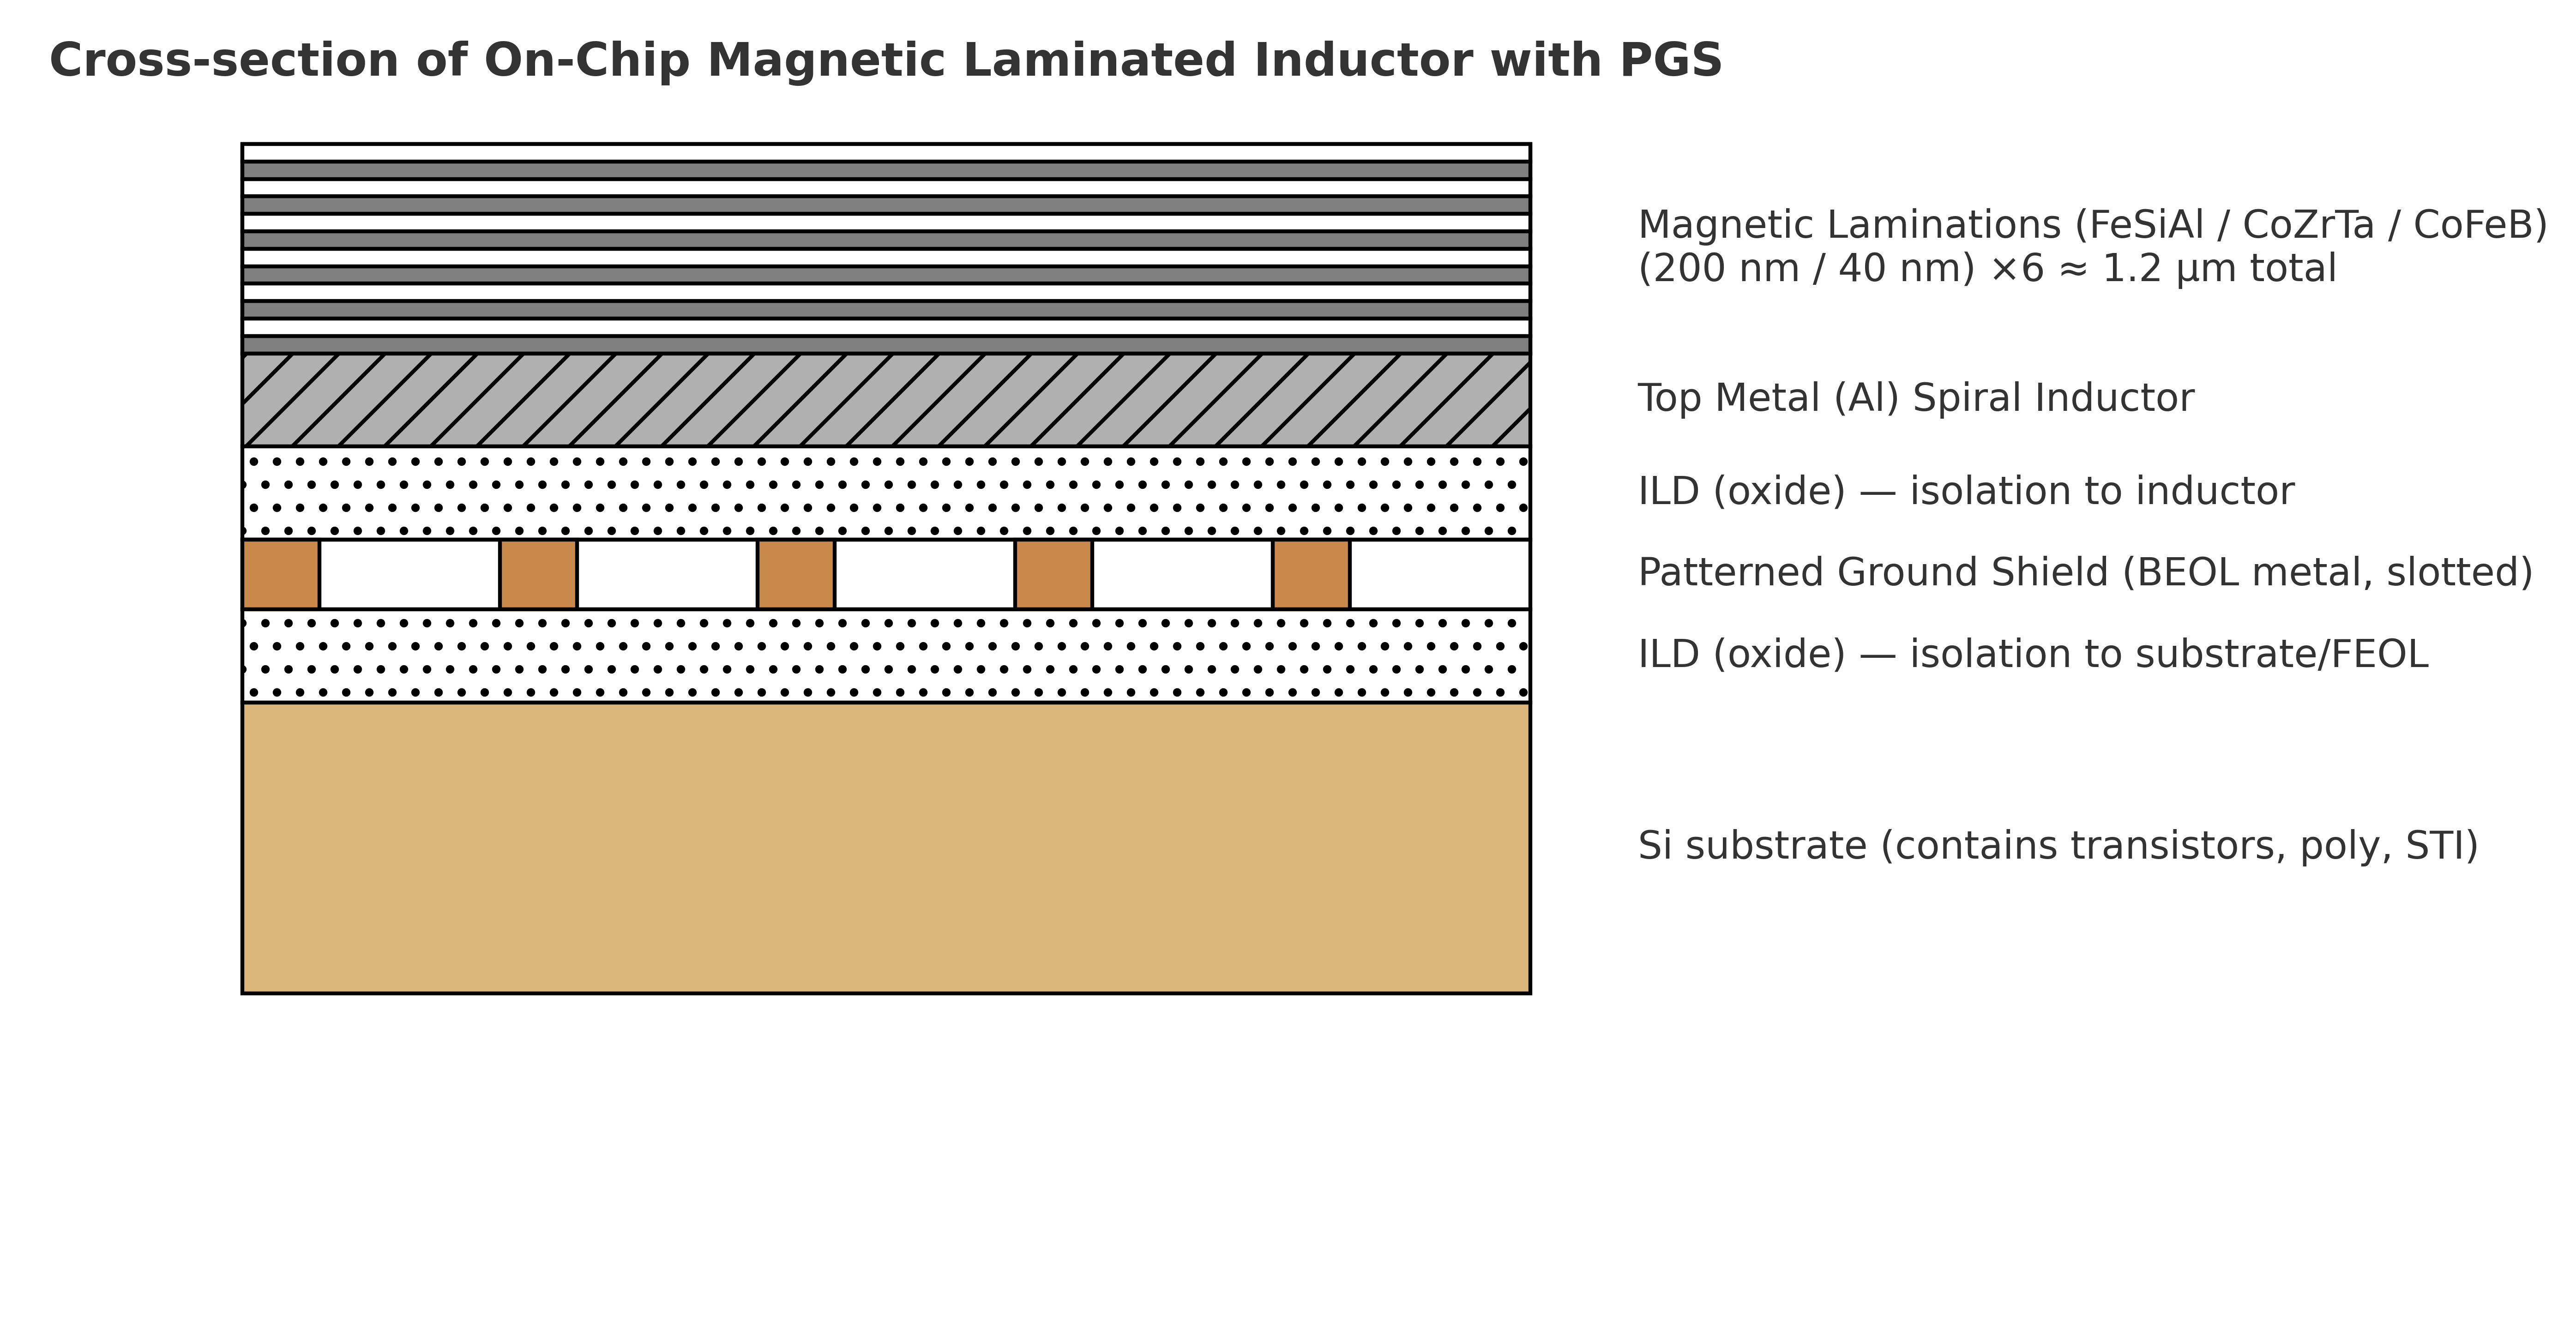
\includegraphics[width=\textwidth]{fig1_laminated_cross_section.png}
  \caption{Cross-sectional concept of the on-chip laminated magnetic inductor with PGS in BEOL.}
  \label{fig:cross_section}
\end{figure*}

\subsection{Patterned Ground Shield}
PGS stripes (8\,µm/24\,µm pitch) reduce substrate losses and improve $Q$ while minimizing eddy currents.

\subsection{Hybrid Buck--LDO Regulator}
The Buck stage provides efficiency, while the LDO attenuates ripple and improves PSRR (Fig.~\ref{fig:buckldo}).

% ===== Fig.2 =====
\begin{figure}[t]
  \centering
  \includegraphics[width=0.9\columnwidth]{fig2_buckldo.png}
  \caption{Hybrid Buck--LDO regulator architecture.}
  \label{fig:buckldo}
\end{figure}

\section{Results}
\subsection{Inductor Performance}
At 20\,MHz, $L=90$--150\,nH, $Q=12$--20, DCR = 0.15--0.25\,$\Omega$, and $I_\text{sat}\geq 0.5$\,A, with 0.6\,mm$^2$ area.

\subsection{Efficiency and Noise}
Hybrid system efficiency reaches 78--82\%. PSRR exceeds 60\,dB at 1\,MHz, with EMI reduced by 3--6\,dB compared to air-core.

% ===== Table I =====
\begin{table}[t]
\caption{Performance summary of air-core vs. proposed laminated inductors.}
\centering
\begin{tabular}{@{}lccc@{}}
\toprule
Metric & Air-core & Proposed & Target \\
\midrule
$L$ (nH) & 40--60 & 90--150 & 100 \\
$Q$ & 3--5 & 12--20 & $>$10 \\
$I_\text{sat}$ (A) & 0.2 & 0.5 & $\geq$0.5 \\
Area (mm$^2$) & 1.2 & 0.6 & -- \\
\bottomrule
\end{tabular}
\label{tab:comparison}
\end{table}

% ===== Fig.3 =====
\begin{figure}[t]
  \centering
  \includegraphics[width=\columnwidth]{fig3_comparison.png}
  \caption{Performance comparison of laminated vs. air-core inductors.}
  \label{fig:comparison}
\end{figure}

\subsection{PSRR Characteristics}
% ===== Fig.4 (full width) =====
\begin{figure*}[t]
  \centering
  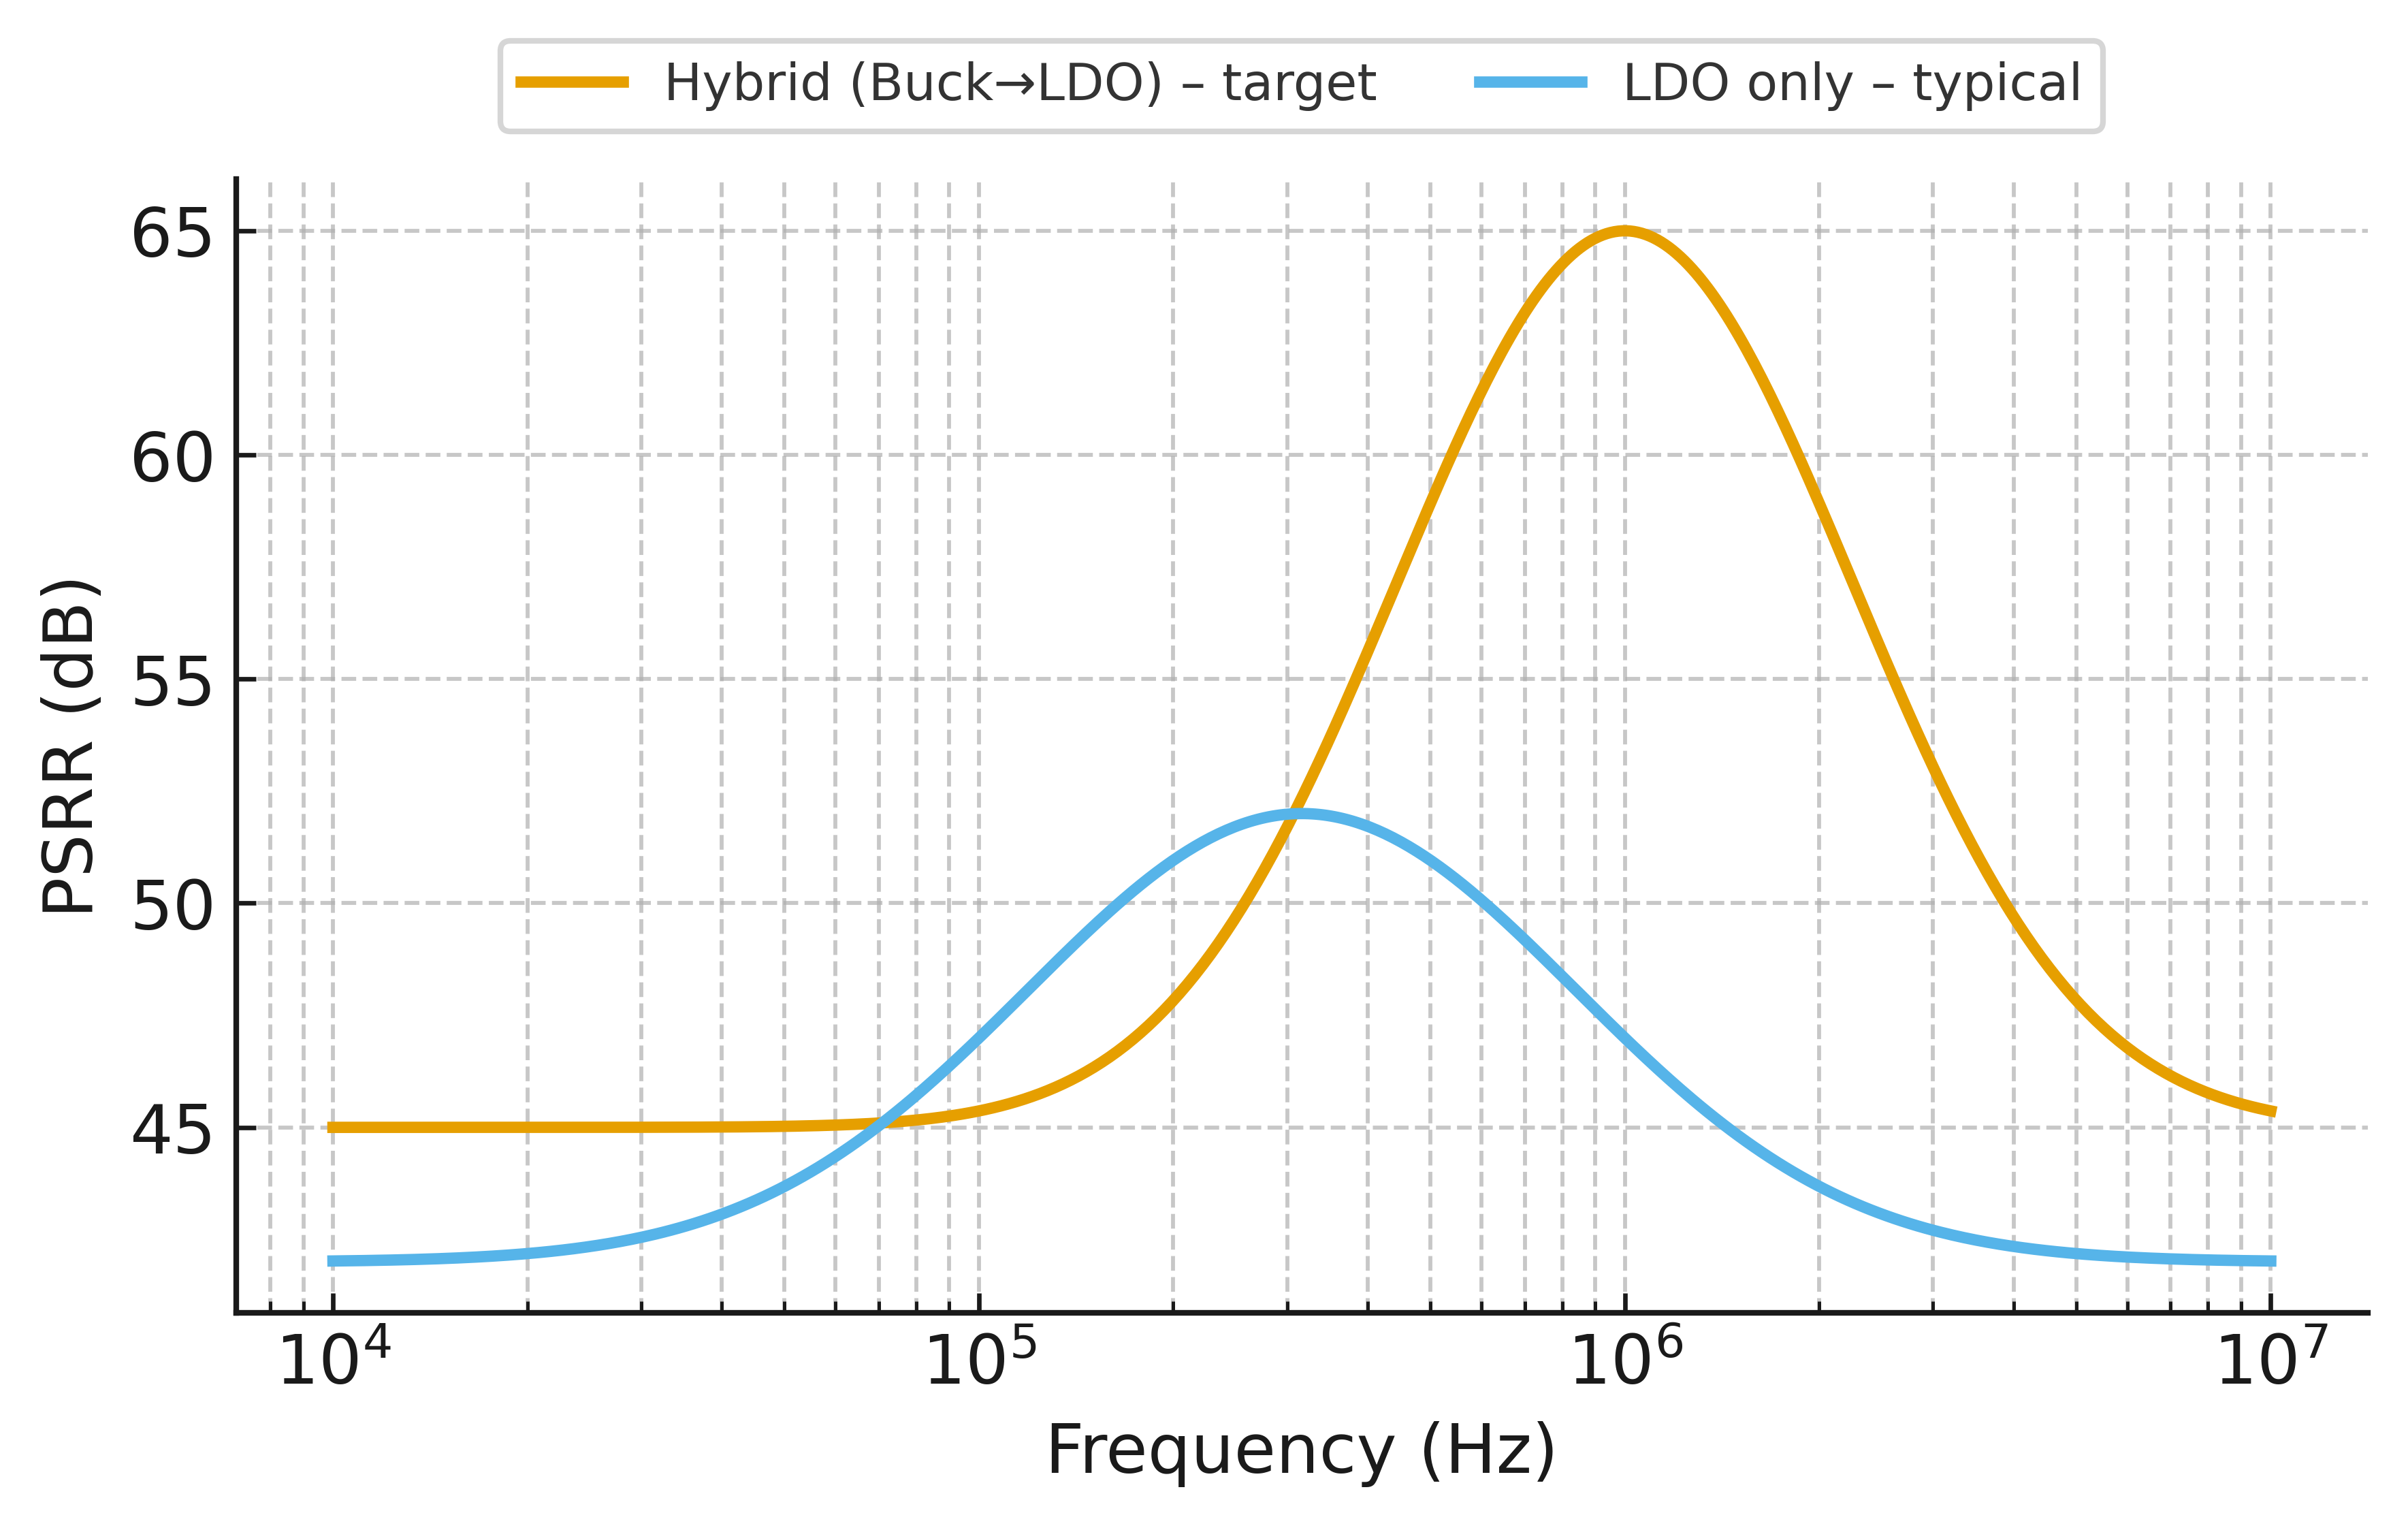
\includegraphics[width=0.95\textwidth]{fig4_psrr_target.png}
  \caption{Target PSRR characteristics of the hybrid Buck--LDO regulator.}
  \label{fig:psrr}
\end{figure*}

\subsection{Transient Response}
% ===== Fig.5 (full width) =====
\begin{figure*}[t]
  \centering
  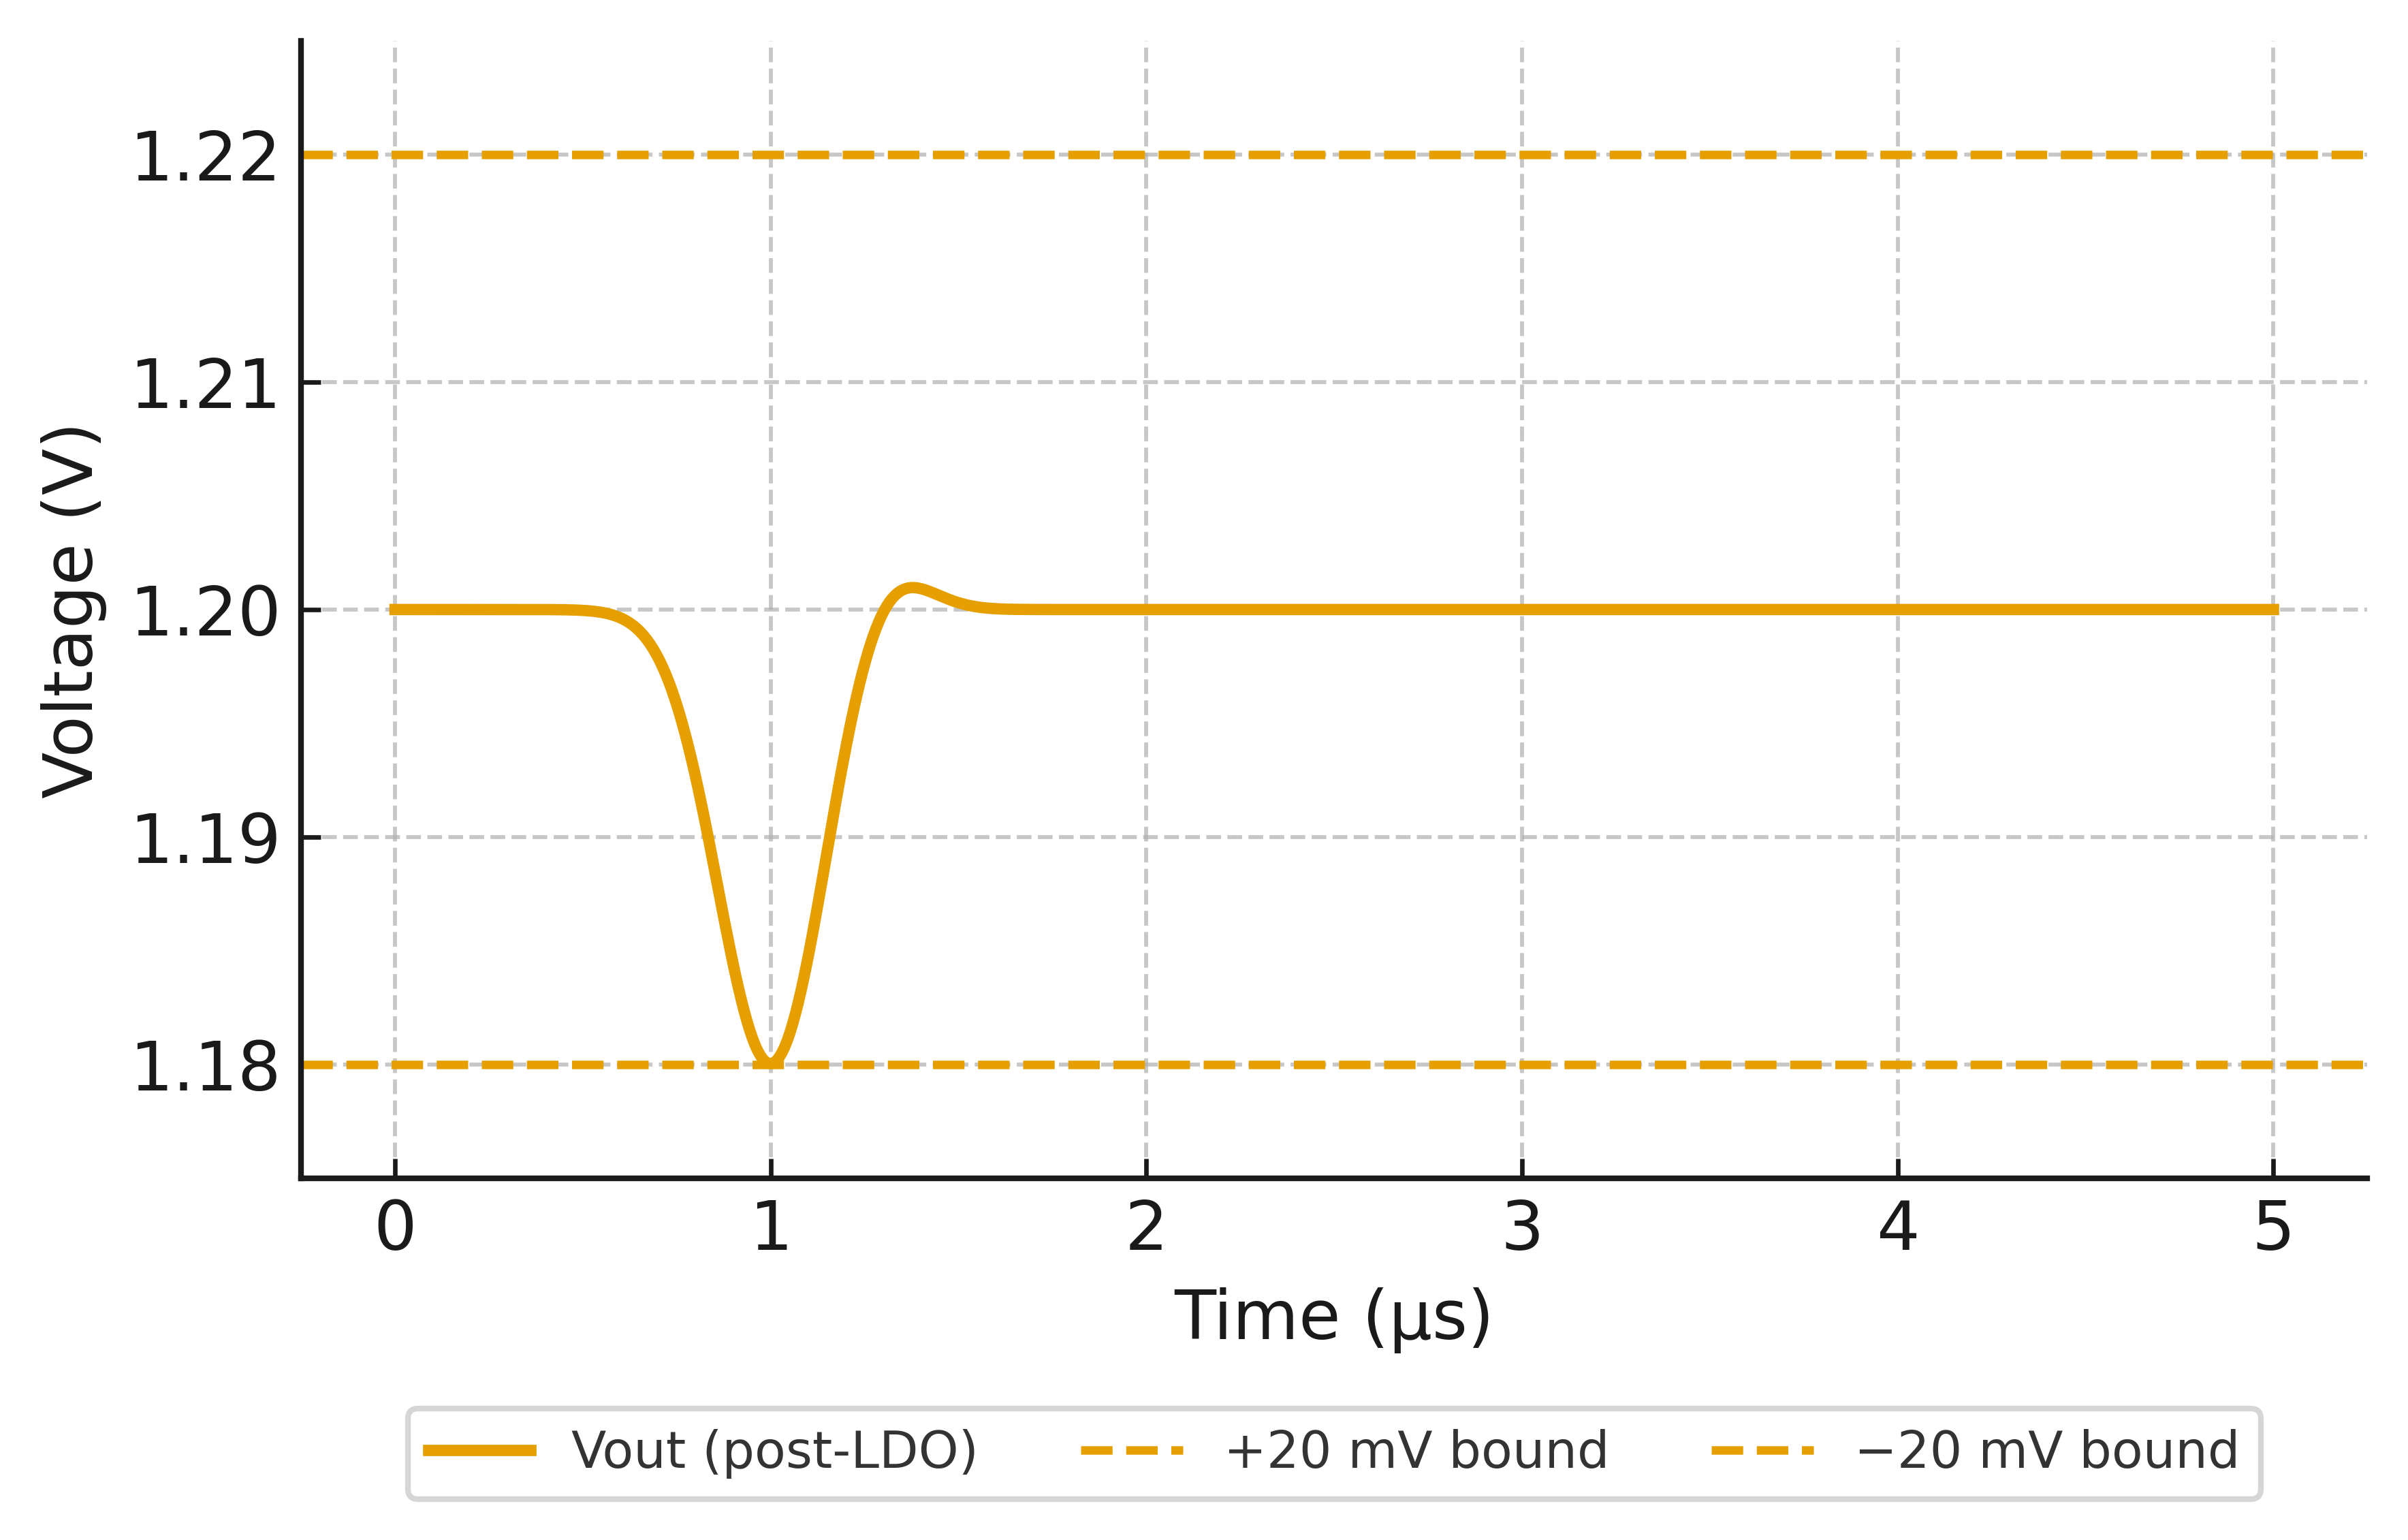
\includegraphics[width=0.95\textwidth]{fig5_transient_response.png}
  \caption{Transient response for a 0.1--0.5\,A load step ($\pm$20\,mV target).}
  \label{fig:transient}
\end{figure*}

\section{Conclusion}
Magnetic lamination with PGS improves inductance and $Q$ while maintaining CMOS compatibility. The hybrid Buck--LDO enables $\approx$80\% efficiency, high PSRR, and fast transient response, suitable for automotive and IoT SoCs.

\section*{Acknowledgment}
The author thanks the Project Design Hub for support.

% ===== References =====
\begin{thebibliography}{10}

\bibitem{ref1}
T. Yachi \emph{et al.}, ``A 20-MHz fully integrated buck converter with on-chip magnetic inductor in 0.18-µm CMOS,'' in \emph{IEEE Int. Solid-State Circuits Conf. (ISSCC)}, pp. 300--301, 2010.

\bibitem{ref2}
J. Park \emph{et al.}, ``High-Q integrated inductors with patterned ground shields in standard CMOS technology,'' \emph{IEEE Trans. Microw. Theory Tech.}, vol. 52, no. 2, pp. 471--478, Feb. 2004.

\bibitem{ref3}
H. Miyake \emph{et al.}, ``On-chip power supply noise reduction using LDO regulator hybrid with switching converter,'' \emph{IEEE J. Solid-State Circuits}, vol. 47, no. 8, pp. 1928--1937, Aug. 2012.

\bibitem{ref4}
K. Makita \emph{et al.}, ``Integrated magnetic thin-film inductors for on-chip power converters,'' \emph{IEEE Trans. Power Electron.}, vol. 28, no. 9, pp. 4384--4394, Sept. 2013.

\bibitem{ref5}
S. Choi \emph{et al.}, ``A 0.18-µm CMOS-compatible FeSiAl magnetic inductor for DC-DC converters,'' \emph{IEEE Electron Device Lett.}, vol. 35, no. 6, pp. 654--656, June 2014.

\bibitem{ref6}
J. Kim \emph{et al.}, ``Low-dropout regulators for SoC applications: Design techniques and trends,'' in \emph{IEEE Custom Integrated Circuits Conf. (CICC)}, pp. 1--8, 2015.

\bibitem{ref7}
A. Elshazly \emph{et al.}, ``An integrated power management system for IoT devices using hybrid Buck-LDO architecture,'' \emph{IEEE Trans. Circuits Syst. I}, vol. 67, no. 10, pp. 3348--3360, Oct. 2020.

\bibitem{ref8}
Y. Kawashima \emph{et al.}, ``High-temperature reliability of thin-film magnetic materials for integrated inductors,'' in \emph{IEEE Int. Rel. Phys. Symp. (IRPS)}, pp. 1--6, 2016.

\bibitem{ref9}
J. Hu \emph{et al.}, ``Advanced magnetic materials for on-chip power inductors: A review,'' \emph{J. Magn. Magn. Mater.}, vol. 491, p. 165621, 2019.

\end{thebibliography}

% ===== Biography =====
\begin{IEEEbiography}{Shinichi Samizo}
received the B.S., M.S., and Ph.D. degrees in electronic engineering. He has been engaged in semiconductor device design, integrated power management, and system architecture for automotive and AI applications. His current interests include on-chip power delivery, control theory, and intelligent design hubs.
\end{IEEEbiography}

\end{document}
